\section{Language Overview}
\label{sec:Overview}

Figure XXX contains a simplified version of CSlang's grammar.  The purpose
of a CSlang program is to completely describe a transducer that both
accepts a chosen stream if it contains a particular
activity sequence and produces an output stream containing specific
modifications needed for application testing.  As a result, such a
description covers all states, their associated output, and the transition
relation that ties them all together.
Simply enumerating every feature of such a transducer could be very verbose
so we carefully tailored CSlang's semantics to allow its users to
describe complex configurations in a concise manner.
We discuss the details of of the
language's syntax and semantics with small examples in
Section~\ref{sub:SyntaxAndSemantics}.  Section~\ref{sub:WorkingExample} walks through a
larger CSlang program explaining each feature along the way.

\subsection{Syntax and Semantics}
\label{sub:SyntaxAndSemantics}

\begin{figure}[H]
\centering
\begin{tabular}{c}
\begin{lstlisting}

S: statementlist
statementlist: statement*
statement: eventdefinition
           | variantdefinition
           | assignment
           | dataword
eventdefinition: id (id\_1, t\_1, l\_1), ..., (id\_n, t\_n, l\_n)
variantdefinition: var\_id ed\_1, ..., ed\_n
assignment: x <- e
dataword: id paramexp predexp outputexp
paramexp: (pid\_1, op\_1, regid\_1), ..., (pid\_n, op\_n, regid\_n)
predexp: (lhs\_1, cmp\_1, rhs\_1), ..., (lhs\_n, cmp\_n, rhs\_n)
outputexp: id paramexp
e \in Expr := e\_1 + e\_2 | e\_1 - e\_2 | ...
\end{lstlisting}
\end{tabular}
\caption{Grammer of CSlang's syntax}
\label{lst:SyntaxGrammar}
\end{figure}


\begin{quote}
\centering
\textbf{S: statementlist}
\end{quote}

This production triggers the creation of a transducer with only a starting
state.  This state is an accepting state in two situations:
\begin{itemize}
  \item{When no other states are added to the automaton by subsequent
    statements}
  \item{When the only other states added to the automaton are NOT states
    which reject sequences where they match the event they describe}
\end{itemize}
In all other cases this is a rejecting state that produces no output.

\begin{quote}
\centering
\textbf{assignment: x <- e}
\end{quote}

Assignment statements store the value of an expression, e, into a named
register on the transducer being described.  If the register does not exist
it is created otherwise its stored value is overwritten.
Registers may contain Numeric or String values.  Register contents
may be used in subsequent statements to specify parameter values that must
be present in order for an event to match or as values to be output.

\begin{quote}
\centering
\textbf{eventdefinition: id (id\_1, t\_1, l\_1), ..., (id\_n, t\_n, l\_n) }
\end{quote}

\preston{ I use the word type here because I can't think of a better term.
I don't like that it could be confused with type as from a type system...}

An event definition statement describes an event that may appear in an input
stream.  Each statement specifies an event ``type'' and a list of
parameters that should be accessible later.  An event's type corresponds
with the system call name, RPC call name, or, in the case of other activity
representations, a unique identifier that would allow events of the same
variety to be picked out of a stream.

\begin{quote}
\centering
\textbf{variantdefinition: var\_id ed\_1, ..., ed\_n}
\end{quote}

A variant definition allows several event definitions to be combined under
a single identifier.  This identifier may then be used in a dataword
statement to match any of the collected events.  This feature arose as a
result of situations where one of several system calls could be used to
perform the same operation (e.g. {\tt read()} and {\tt recv()}).

\begin{quote}
\centering
\textbf{dataword: id paramexp predexp outputexp}
\end{quote}

Dataword statements are responsible for adding new states to the
transducer.  This means they must specify any register operations,
transition conditions, and output associated with these new states.  To
tackle this complexity we will address each part of this production
individually.

\textit{id paramexp}

The parameter expression offers an opportunity to examine and store
parameter values from the current event.  CSlang supports two operators
that may be applied to parameter expression members.  The match operator
(!) allows for the rejection of otherwise matching events
by enforcing a required value on a
chosen parameter while the store operator (?) copies a value from the
current event and stores it in the specified register.


\textit{predexp}

Predicate expressions are used to place additional restrictions that must
be met if the transducer is to advance into the newly created state.  These
restrictions compare values from the current event to either register
values or literal values.

\textit{outputexp}

An output clause controls the output that will be produced when its
associated state is entered.  The nature of this output is controlled by a
parameter expression which specifies which parameters of the current event
should be replaced with a value from a register.  If a parameter is not
included in the parameter expression, its original value is used and,
similarly,
if an output clause is omitted the original, unmodified event is output.

\subsection{Dataword Operators}
\preston{I don't know if we need to discuss these further or if the above
is enough to cover them}
\textit{Match Operator (?)}

\textit{Store Operator (!)}


\subsection{Other Features}
\preston{I don't know if this is worth its own subsection}
\textit{The NOT Keyword}



%%%% We need to talk about how we are different from other
%%%% languages that are regular-expression like here
%\subsection{Inspiration from Regular Expressions}
%
%
%%%% This is probably better called something more generic like "type
%%%% system" because we also have variant types and need to describe why we
%%%% included them and how they help us express stuff
%\subsection{Record Data Types}
%
%some messages support parameters with complex data types.  As a
%result.........
%
%\subsection{Intermediate Data Format and Message Adapter Classes}
%
%Ensuring CSLang was easy to extend is a central concern.  We provide an
%intermediate data format as well as a description of how to construct
%message format adaptors cthat transform messages into it.........
%
%\subsection{Register Operations}
%
%Many interesting anomalies require modifications to data that occurred
%earlier in the trace...  Need expressions that can do these manipulations
%and output them.....
%
%
%\subsection{Nuts and Bolts}
%CSLang's tooling consists of AAA lines of Python code.
%\begin{itemize}
%\item{Parser written using PLY}
%\item{Compilation results in a pure-python object serialized to disk}
%\end{itemize}
%
%\subsection{Using CSLang}
%
%Using CSLang is a familiar process to anyone who has written, compiled, and
%executed code from another programming language....
%
%\begin{enumerate}
%\item{Anomaly is identified}
%\item{Anomaly is described using CSLang}
%\item{Anomaly is compiled into a transducer}
%\item{Transducer is executed on a stream of incoming syscalls, rpc calls, etc}
%\item{Mutated calls come out the other end}
%\item{Application being tested is exposed to simulation of mutated calls}
%\begin{itemize}
%\item{This is CrashSimulator for system calls}
%\item{Some other tool for RPC applications}
%\end{itemize}
%\item{Results come out the other side}
%\end{enumerate}
%
%\subsection{The Anatomy of a CSlang Program}
%
%\begin{figure}
%  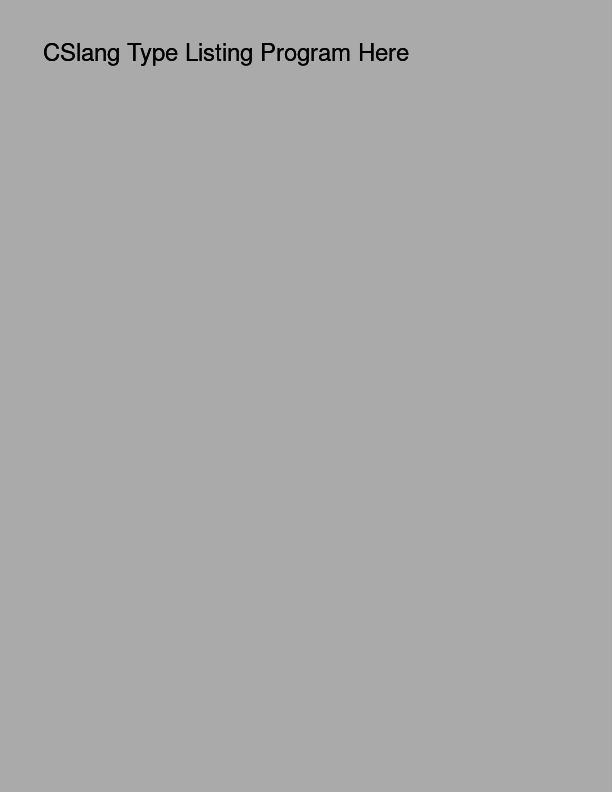
\includegraphics[scale=.30]{images/typelisting}
%  \caption{}
%  \label{fig:typelisting}
%\end{figure}
%
%\begin{figure}
%  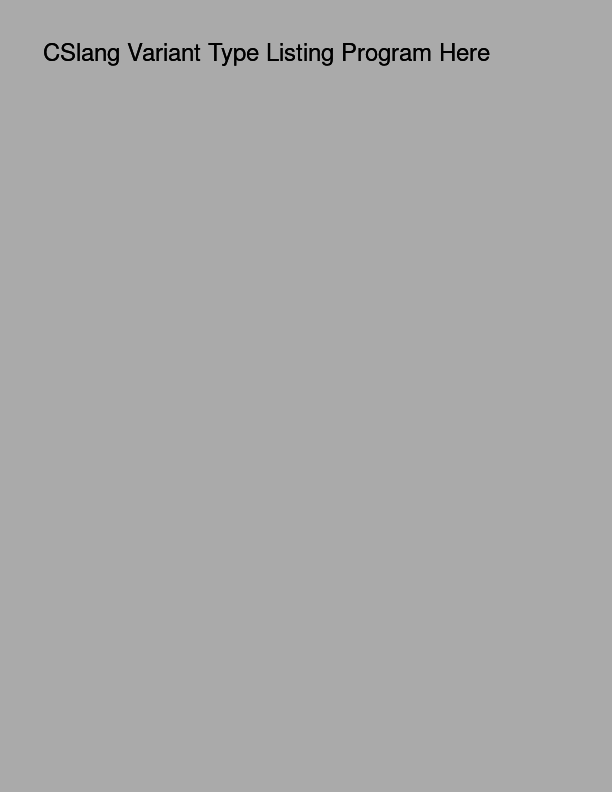
\includegraphics[scale=.30]{images/varianttypes}
%  \caption{}
%  \label{fig:varianttypes}
%\end{figure}
%
%Figure~\ref{fig:bigprogram} shows a complete CSlang program that matches,
%and allows for the manipulation of, a sequence of system calls that
%facilitates the retrieval of data from a webserver and its storage to a
%file on disk.  Such a sequence may be found in programs like {\tt wget} or
%{\tt curl}.
%
%Lines 1 through 4 of this program define constructors for the types, {\tt
%socket}, {\tt connect}, {\tt send}, {\tt recv}, {\tt read}, and {\tt
%write}.  Each of these types corresponds to a system call involved in the
%target sequence and the system call parameters we will used to refine the
%specific calls to be matched from a system call listing.
%
%
%Lines 6 through 10 define each define a transducer state that may only be
%entered upon encountering a system call with parameters matching the values
%defined in the statement....
%
%
%Figure~\ref{fig:varianttypes} shows an analogous program to the one show in
%figure~\ref{fig:bigprogram}.  The purpose of this second program is to
%illustrate how CSlang's variant types can be used to more flexibly define a
%sequence of system calls.  This is particularly useful when a given task
%can be accomplished by more than one system call.  For example, consider
%the type {\tt allread} defined on line XXX.  Whenever a statement defines a
%state that accepts allread it may be entered upon encountering either a
%{\tt read} or {\tt recv} call as these system calls may both be used to
%read data from a socket file descriptor (though with slightly different
%parameters).  A similar situation can be observed with the type {\tt
%allselect}.  Statements accepting allselect may be entered with any of {\tt
%poll}, {\tt epoll}, or {\tt select}.  By defining these types in this
%manner, a program can be constructed to accept a wider range of sequences
%that are all performing the same operation described the first program but
%using different system calls.
